\documentclass[12pt, a4paper]{report}
\usepackage{graphicx}
\usepackage[english]{babel}
\usepackage{amsthm}
\usepackage{amssymb}
\usepackage{amsmath}
\usepackage{algorithm}
\usepackage{algpseudocode}

\newtheorem{theorem}{Theorem}[section]
\newtheorem{corollary}{Corollary}[theorem]
\newtheorem{lemma}[theorem]{Lemma}
\theoremstyle{remark}
\newtheorem*{remark}{Definition}

\title{Uncertainty In Artificial Intelligence\\ \textit{Theory}}
\author{Christian Rossi}
\date{Academic Year 2023-2024}

\begin{document}

\maketitle

\newpage

\begin{abstract}
    The topics of the course are:
    \begin{itemize}
        \item Uncertainty sources that acffect models: typology, issues, and modeling approaches.
        \item Measure-based uncertainty modeling.
        \item Logic-based uncertainty modeling.
        \item Fuzzy models: fuzzy sets, fuzzy logic, fuzzy rules, motivations for fuzzy modeling, tools for fuzzy systems, design 
        of fuzzy systems, applications.
        \item Bayesian networks: basics, design, learning, evaluation, applications.
        \item Hidden Markov Models: basics, design, learning, evaluation, applications.
        \item Applications: motivations, choices, models, case studies.
    \end{itemize}
    \end{abstract}

\newpage

\tableofcontents

\newpage

\chapter{Introduction}
    \section{Definition}
    \begin{remark}
        \emph{Uncertainty} refers to epistemic situations involving imperfect or unknown information. It applies to predictions 
        of future events, to physical measurements that are already made, or to the unknown. 
    \end{remark}
    Uncertainty arises in partially observable or stochastic environments, as well as due to ignorance, indolence, or both. It arises 
    in any number of fields, including insurance, philosophy, physics, statistics, economics, finance, medicine, psychology, sociology, 
    engineering, metrology, meteorology, ecology and information science.
    
    The lack of certainty, a state of limited knowledge where it is impossible to exactly describe the existing state, a future outcome,
    or more than one possible outcome. This puts in evidence that uncertainty is related to the need of describing a piece of reality.

    \section{Modelling}
    Modelling is at the base of our life: the way we interact with the world is through models that interpret data coming from sensors
    and generate knowledge and actions. Modelling is also the way we may represent entities in a computer and possibly making it reasoning
    on them.
    \begin{remark}
        A \emph{model} is a representation of some entity, defined for a specific purpose. A model captures only the aspects of the entity
        modelled that are relevant for the purpose. A model is necessarily different from the modelled entity. So, intrinsic to modelling
        are all sort of uncertainities.
    \end{remark}
    All Artificial Intelligence applications are based on models, either defined by somebody or learned. Thes models are represented In
    different ways, but share uncertainty issue mainly on inputs. 

    \section{Uncertainty classification}
    The uncertainty can be of two main types: 
    \begin{itemize}
        \item Epistemic uncertainty: it is due to things one could in principle know but does not in practice. This may because a 
            measurement is not accurte, because the model neglets certain effects, or because particular data have been deliberately
            hidde. It is also known as systematic uncertainty and can in principle be reduced by enriching the model.      
        \item Aleatoric uncertainty: it is representative of unknown unknowns that differ each time we run the same experiment. 
            Aleatoric uncertainty is also known as statistical uncertainty, since only statistical information can describe it. This may
            also depend on the way we get and elaborate data. In general it is present when the model is missing some aspects.
    \end{itemize}
    The sources of uncertainty can be: 
    \begin{itemize}
        \item Parameter: it comes from the model parameters, whose esact values are unkonwn to experimentalists and cannot be controlled
            in experiments, or whose values cannot be inferred by statistical methods. 
        \item Parametric variability: it comes from the variability of input variables of the model. 
        \item Structural: also known as model inadequacy, model bias, or model discrepancy, this comes from the lack of knowledge of the
            problem.
        \item Algorithmic: also known as numerical uncertainty, or discrete uncertainty. This type comes from numerical errors and
            numerical approximations in the implementation of the computer model. 
        \item Experimental: also known as observation error, this comes from the variability of experimental measurements.
        \item Interpolation: this comes from a lack of variable data collected from computer model simulations and/or experimental 
            measurements. 
    \end{itemize}

    \section{Uncertainty modelling}
    The type of uncertainty model depends on the type of uncertainty, its sources and the information we have in uncertainty and mostly
    has to do with qualification and quantification of uncertainty. The possible model for uncertainty are: statistical, logical and
    cognitive.

    Artificial Intelligence and Machine Learning technlogies are based on models that include uncertainty models of these sorts, essential
    not only for the implementation of effective models, but also to define learning models able to cope with complex situations, and 
    to evaluate the quality of learned/developed models. 
    There are two major types of problems in uncertainty quantifiaction: 
    \begin{itemize}
        \item Forward propagation of uncertainty: the various sources of uncertainty are propagated through the model to predict the overall
            uncertainty in the system response:
            \begin{itemize}
                \item To evaluate low-order moments of the outputs (mean and variance).
                \item To evaluate the reliability of the outputs.
                \item To assess the complete probability distribution of the outputs. 
            \end{itemize}
            This is what is done also in Bayesian Networks and Graphical models. 
        \item Inverse assessment of model uncertainty and parameter uncertainty, where the model parameters are calibrated simultaneously
            using test data: given some experimental measurements of a system and some results from ist mathematical model, inverse 
            uncertainty quantifiaction estimates the discrepancy between the experiment and the mathematical model (bias correction) and
            estimates the values of unknown parameters un the model if there are any (parameter calibration).
    \end{itemize}
    The models used in Artificial Intelligence can be classified in three main types: 
    \begin{itemize}
        \item Symbolic models: elements of the models are expressed as terms related to entities to be modelled. The state of the world is
            represented by facts expressed in formal languages close to natural languages.
        \item Sub-symbolic models: elements of the models are expressed by code. 
        \item Black-box models: the model can be computed and possibly investigated, but it is only regarded as a computational way to map
            inputs to outputs. 
    \end{itemize}
    For symbolic models a fact is true in a model if it is possible to collect enough evidence to support it. the only really true facts 
    are the ones true by definition. All the others may be supported by evidence. 
    
    \section{Ignorance management}
    There are many potential sources of ignorance when reasoning in the real world:
    \begin{itemize}
        \item Insufficient data.
        \item Biased data: data are collected by sensors affected by errors. 
        \item Variable data: data are collected by imprecise sensors.
        \item Reliability of data. 
        \item Fuzzyness. 
        \item Reliability of the model: depends on the model design, implementation and parametrization. 
        \item Incompleteness of the model. 
    \end{itemize}
    \begin{figure}
        \centering
        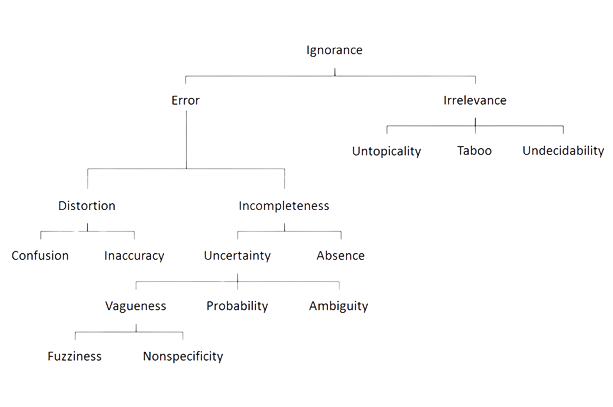
\includegraphics[width=1\linewidth]{images/smithson.png}
        \caption{Smithson's taxonomy of ignorance and uncertainty}
    \end{figure}
    To model ignoranche most often it is decided to associate measures of some aspects. Let's distinguish between two aspects: 
    \begin{itemize}
        \item The type of representation: numbers, labels, intervals, \dots
        \item The represented ignorance thet we would like to model: i.e, probability, reliability, subjective evaluation, \dots
    \end{itemize}

    The probability is represented with numbers between zero and one, and a well-established set of rules and properties are associated 
    to its management, among which, given a set of alternative hypotesis: 
    \begin{itemize}
        \item The sum of their probabilities should be one. 
        \item The probability a posteriori of a hypotesis $h_i$ given some evidence $e$ si given by the Bayes theorem:
            \[P(h_i \mid e)=\frac{P(e \mid h_i)P(h_i)}{P(e)}\]
    \end{itemize}
    Probability was used, for example, in the MYCIN that was one of the first expert systems, aimed at diagnosing blood illness. They 
    modeled certainty by considering two numerical factors: 
    \begin{itemize}
        \item Measure of increased Belief: $MB=\frac{P(\frac{h}{e})-P(h)}{1-P(h)}$.
        \item Measure of decreased Disbelief: $MD=\frac{P(h)-P(\frac{h}{e})}{P(h)}$.
    \end{itemize}
    The measure of a statement is given by the certain factor:
    \[CF=MB-MD \in [-1;1]\]
    The main hypotesis for this solution is that the number given as $MB$ and $MD$ are not statistical probabilities, but subjective
    probabilities, provided by different experts and combined by rules (this may be ambiguous). 

    Compared to probabilities, linguistic terms are less ambiguous than numbers. Unsing a limited set of labels it is possible to associate
    to statements subjective evalutations, on which it is relatively easy to make subjective judgements converge. Then, a computational 
    mechanism is needed to define how to combine labels. This is done by using fuzzy systems, that are a representation of truth  of a 
    statement in linguistic terms, as evaluation of its fuzzyness. 

    \newpage

    \chapter{Fuzzy systems}
\end{document}